\chapter{Implementation}
\label{chap-3:implementation}

\section{Data collection}

Quality of any machine learning model very strongly correlates with quality and quantity of the input data.
In this project, input data are features \ref{chap:features} computed from the GitHub repositories\footnote{See \url{https://docs.github.com/en/github/creating-cloning-and-archiving-repositories/about-repositories}}.

\begin{figure}
    \centering
    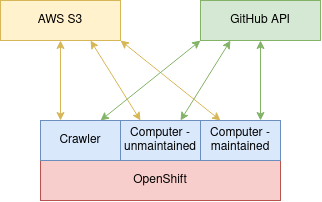
\includegraphics[scale=0.9]{chapters/chapter3/architecture.png}
    \caption{Data gathering architecture, Source: own}
    \label{fig:architecture}
\end{figure}

Figure \ref{fig:architecture} illustrates the data gathering process.
Three containers: \emph{crawler} \ref{sec:crawler}, \emph{computer - unmaintained} and \emph{computer - maintained} \ref{sec:computer} are running on the \emph{OpenShift} \ref{sec:openshift} platform.
Containers store and load data from the \emph{S3} storage \ref{sec:s3} and make calls to the \emph{GitHub API}.

\subsection{Tools used for data collection}

\subsubsection{Containers}
\label{sec:containers}

Containers contain a runtime environment which comprises the software application, its dependencies, libraries, binaries and configuration files.
The software application runs on the container and does not depend on the host environment except for the operating system.
A container can contain multiple apps and each app will have its own environment\footnote{See \url{https://www.techopedia.com/2/31967/trends/open-source/container-technology-the-next-big-thing}}.
Containerization thus provides a lightweight, isolated environment that makes apps easier to deploy and manage.

\begin{figure}
    \centering
    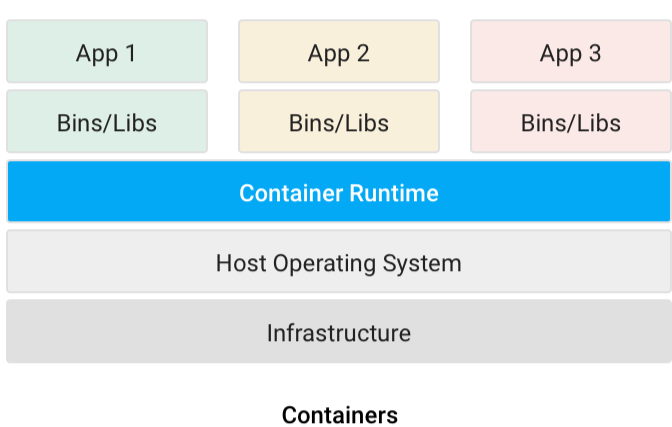
\includegraphics[scale=0.5]{chapters/chapter3/containerization.png}
    \caption{Container architecture\footnote{See \url{https://cloud.google.com/containers}}}
    \label{fig:container}
\end{figure}

Figure \ref{fig:container} shows the schema of a container architecture.
Applications \emph{App 1}, \emph{App 2} and \emph{App 3} are bundled with their dependencies and running on the \emph{container runtime}, software responsible for running containers.
\emph{Container runtime} runs on the host operating system which runs on the underlying infrastructure.

Running data collection components \ref{sec:crawler} and \ref{sec:computer} as containers has allowed me to take advantage of an Red Hat's OpenShift \ref{sec:openshift} cluster.

\subsubsection{OpenShift}
\label{sec:openshift}

Red Hat OpenShift\footnote{See \url{https://www.redhat.com/en/technologies/cloud-computing/openshift}} is an enterprise-ready Kubernetes\footnote{See \url{https://kubernetes.io/}} container platform.
It functions as a Platform-as-a-Service\footnote{See \url{https://www.oracle.com/cloud/what-is-paas/}} and a Container Orchestration\footnote{See \url{https://www.vmware.com/topics/glossary/content/container-orchestration}} Engine.

In the simplest of terms, it provides a platform for running and managing containers \ref{sec:containers}.
OpenShift is focused on a security on every level of a container stack, it also provides a huge set of other functionalities\footnote{See \url{https://www.openshift.com/}} including automated installation, upgrade, lifecycle manager and others.

\subsubsection{Amazon S3}
\label{sec:s3}

Data collection process is carried out by applications running as containers \ref{sec:containers}.
These applications generate data that need to be stored in the permanent storage outside of the containers.
\emph{Amazon S3}\footnote{See \url{https://aws.amazon.com/s3/}} provides such storage.

Amazon Simple Storage Service (Amazon S3) is an object storage service that offers industry-leading scalability, data availability, security, and performance.
Customers of all sizes and industries can use it to store and protect any amount of data for a range of use cases, such as data lakes, websites, mobile applications, backup and restore, archive, enterprise applications, IoT devices, and big data analytic\footnote{See \url{https://aws.amazon.com/s3/}}.

\subsection{Searching for suitable repositories}

\subsubsection{Filtering repositories}
\label{sec:filtering}

In the time of the study GitHub offers more than 38 million public repositories\footnote{See \url{https://github.com/search?q=is\%3Apublic\&ref=simplesearch}}.
Not all of them are suitable for this study, there are three minimal requirements repositories have to meet.

\begin{enumerate}
    \label{sec:suitable}
    \item \emph{Development time} \ref{feature:development_time} of more than 730 days (two years).
    Several features \ref{chap-3:features} require historical data.
    Idea behind is that estimating a longevity based on couple of weeks of development would be very inaccurate.
    % todo pidat citacie papierov kde brali featury z poslednych dvoch rokov vyvoja
    Several other studies used a similar time frame for evaluating repositories \cite{}.

    \item Repository contains a code in a programming language.
    Considerable portion of repositories do not contain files in a programming language.
    Examples are projects providing resource lists, CSS\footnote{See \url{https://developer.mozilla.org/en-US/docs/Learn/CSS/First\_steps/What\_is\_CSS}} templates or a content in some other markup or data type language.

    \item Project started a development using \emph{git} version control system.
    Some projects on GitHub were initially using some other version control\footnote{See \url{https://en.wikipedia.org/wiki/Template:Version\_control\_software}} and ported to \emph{git} in a later stage of the development.
    This devalues the data as the whole development process before the transition is squashed into a single or few commits, which do not realistically represent the full process from the start.

    A project is considered to be started outside of GitHub and then transitioned there later if more than 50\% of files were added in less than 20 commits.
    Same method is used in \cite{p:16}.

\end{enumerate}

Repositories satisfying previous criteria are considered suitable for the study.
Such projects are then divided into two categories.

\begin{enumerate}
\label{sec:(un)maintained}
    \item Unmaintained: there are three criteria necessary for unmaintained repositories:
        \begin{enumerate}
            \item Repository is archived\footnote{See \url{https://docs.github.com/en/github/creating-cloning-and-archiving-repositories/archiving-a-github-repository}}.
            Repository owners can archive their repositories to make it read-only and to let people know that the project will no longer be maintained.
            This is far better alternative to just deleting the repository, as users can still fork and use the archived projects.
            It would be very convenient for this study, if every unmaintained project was marked as archived.
            This is not the reality.
            While archiving projects that are no longer under active development is considered a good practice, it is not required.
            
            \item In some cases, repository owner puts the information about the end of development into the \emph{README} file.
            The crawler scans this file and marks a repository unmaintained if any of the following keywords is found: \emph{deprecated}, \emph{unmaintained}, \emph{no longer maintained}, \emph{no longer supported}, \emph{no longer under development}, \emph{not maintained}, \emph{not under development}, \emph{obsolete}, \emph{archived}.

            In some instances, such keyword can be used for some other purpose than to let the reader know that the project is no longer being developed.
            There are ... repositories classified as \emph{unmaintained} because of the found keyword in the README.
            For this reason, I manually checked all of such repositories to confirm if the repository was classified correctly.
            In the case of misclassification because of keyword used in some other context, said repository was reclassified correctly.
            Process was similar as in \cite{p:8}.

            \item Last criterion is that the last commit was submitted more then a year (104 weeks) ago.
            No activity for a year is a clear sign that the project's community is no longer continuing the development of the project.
        \end{enumerate}

    \item Maintained: suitable projects not considered unmaintained are viewed as maintained.
\end{enumerate}

Searching through repositories and their consecutive classification to not suitable/suitable and unmaintained/maintained is done by a \emph{crawler}.

\subsection{Developed applications}
\label{sec:applications}

\subsubsection{Repositories crawler}
\label{sec:crawler}

I created a crawler program to go through GitHub repositories and classifies \ref{sec:filtering} them.
Crawler goes through repositories in a random fashion.
The process is as follows:

\begin{enumerate}
    \item User selects a range of years for the crawler to search through.
    Repositories created within this time range will be considered for crawling.
    Input is added thru the configuration file \ref{sec:input}, the default search range and the one used for the study is years \emph{2009 - 2019}.
    Because of the \emph{suitability} requirement \ref{sec:suitable} of two years worth of historical data, the upper bound of this range is set to 2019.
    Repositories created after 2019 naturally do not have enough data to be fitting for the study.
    Lower bound is chosen arbitrarily.

    \item Time range is then transformed into an ID range.
    Repository IDs are represented as integers.
    Values of IDs of newly created repositories are higher than values of IDs of previously created repositories.
    This is convenient, as it can be exploited to make a random crawling of repositories easier.
    Transformation from a time range to an ID range is as follows:
    
    \begin{enumerate}
        \item Lower bound of an ID range is an ID of the first repository created in the year given by the lower bound of a time range.
        \item Upper bound of an ID range is an ID of the first repository created in the year given by the upper bound of a time range.
    \end{enumerate}

    \item Crawler that chooses an integer from the ID range with the uniform probability\footnote{Method used for this step of the process is \emph{random.randrange}, see \url{https://docs.python.org/3/library/random.html\#random.randrange}}.
    Not all IDs within the range still represent an existing repository, so the crawler needs to check the validity of the chosen integer.
    If the generated integer is a valid ID, process proceeds to the next step, if it is not, than it chooses another integer.

    % todo "vysiaca" referencia
    \item In the last step, the crawler classifies the repository \ref{sec:filtering} and saves the ID into the corresponding file.
\end{enumerate}

\subsection{Features computer}
\label{sec:computer}

Once the \emph{crawler} \ref{sec:crawler} gathers IDs of suitable repositories, another program, \emph{computer}, can compute the requested features of the repositories.
\emph{Computer} will go through the IDs collected by the \emph{crawler}.
For every ID, it will compute all of the implemented features specified in the \emph{configs/data\_gathering/features.yml} file \cite{repo}.

\subsection{Features of crawler and computer}

Although responsible for different tasks, both programs crawler and computer work in a very similar way.
They were both created with the same goals in mind.
Here are some notable features.

\subsubsection{Extensibility}

I proposed a set of features \ref{chap-3:features} to be used for the study.
New features can be added quickly:
they need to be implemented in the \emph{data\_gathering/repository\_data.py} and then referenced in the \emph{configs/data\_gathering/features.yml} file.

Extensibility is important, as it allows different users with different use cases to easily shape \emph{crawler} and \emph{computer} to better meet their specific needs.

\subsubsection{Scalability}

Project contains three \emph{Dockerfiles}\footnote{See \url{https://docs.docker.com/engine/reference/builder/}} for a \emph{crawler}, a \emph{computer} of unmaintained repositories and a \emph{computer} for maintained repositories.
These \emph{Dockerfiles} can be used to build containers \ref{sec:containers} which can be run on a container platform\footnote{See \url{https://en.wikipedia.org/wiki/OS-level_virtualization\#Implementations}}.
Users with sufficient resources can scale up a number of these containers and gather the data at a faster rate.

In the case of this project, applications were running as containers in the OpenShift cluster \ref{sec:openshift} provided by Red Hat\footnote{See \url{https://www.redhat.com/en}}.

\subsubsection{Flexibility}

Data gathering of on a sufficient scale takes up hundreds of hours.
The whole process does not need to finish in the single run.
Applications \emph{crawler} and \emph{computer} are build in such way that their computation can be terminated without the loss of previously computed data.

Both programs periodically and at the end of the execution serialize all of the computed data and upload them to the specified permanent storage.
At the beginning of the executions, both programs first check for the existing data in the permanent storage.
When preceding data is detected, applications will download them, unpack and then carry on with the computation.
Frequency of periodic saves and uploads of the data can be adjusted via a configuration file\footnote{See \url{https://github.com/samuelmacko/master\_thesis/blob/master/configs/data_gathering/gathering.yml}}.
Solution for the permanent storage used for this project is \emph{AWS S3} \ref{sec:s3}.

This alleviates the danger of losing potentially hours worth of computed data, in an event resulting in an application termination.
Containers can also be shut down, rebuild and re-run in order to update the application.

\subsubsection{Logging}

Both programs, \emph{crawler} and \emph{computer}, make use of detailed logging.
Log files are uploaded to the persistent storage with the other data.
This is useful in case of Pod\footnote{See \url{https://kubernetes.io/docs/concepts/workloads/pods/}} crashes which leave no Pod log file available.
Logs also inform about the progress of the data gathering and feature computation.

There are two levels of logging, NORMAL and DEBUG.
NORMAL level is mainly for displaying the progress, DEBUG on the other hand, shows more exhaustive progress information and possible errors.

\section{Dataset}

For the thesis, ... suitable \ref{sec:suitable} repositories were gathered.
Of these ... were classified as \emph{maintained} and the rest -- ... -- as \emph{unmaintained} \ref{sec:(un)maintained}.
\emph{Maintained} projects make only ...\% of all of the suitable repositories.
This small sample of all of the GitHub repositories indicates, that only a smaller fraction of them are under an active maintenance.

One of the conditions for the repository to be classified as \emph{unmaintained} is one of the selected keywords present in the \emph{README} file.


\section{Removing highly correlated features}

A dataset sample consists of 28 features \ref{chap-3:features}. 
I removed highly correlated features using \emph{Pearson correlation coefficient}\footnote{See \url{https://en.wikipedia.org/wiki/Pearson_correlation_coefficient}}.
Threshold for the removal is set to 90\%, sufficiently correlated -- and thus removed -- features are:

\begin{itemize}
    \item issues\_count\_open
    \item issues\_count\_closed
    \item releases\_count
    \item stargazers\_count
    \item wealth
\end{itemize}

Correlation heatmap can be seen in the figure \ref{fig:heatmap}.
Final number of features is then 23.

\begin{figure}
    \centering
    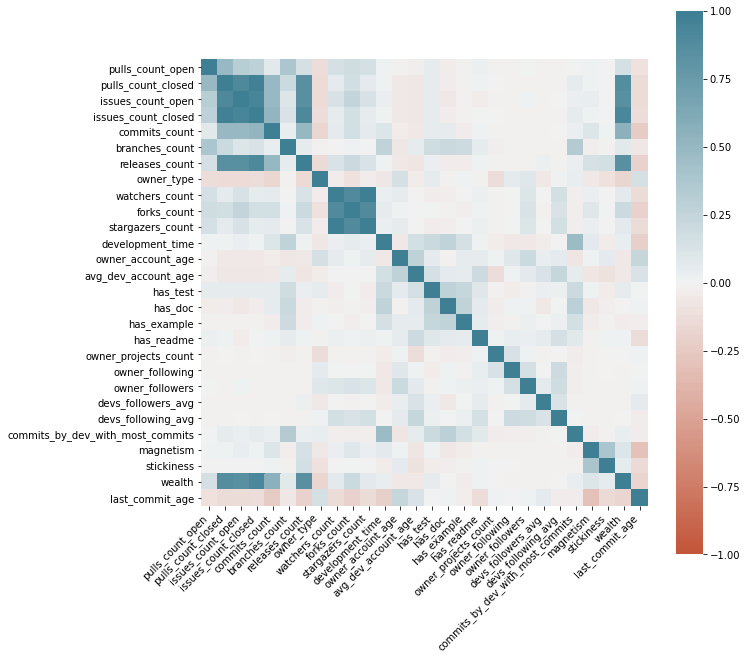
\includegraphics[scale=0.5]{chapters/chapter3/corr-heatmap.png}
    \caption{Correlation heatmap}
    \label{fig:heatmap}
\end{figure}

% todo nejake grafy descriptive statistics
% mean, standard deviation, skewness, quartiles niektorych featur
% kolko ma readme, testy a take veci
% vizualizacia: boxploty pre mean, variance, ...
% "podozrive" featury na korelaciu overit aj statistickymi testami a potom nepouzivat v datasete

\section{Dataset preprocessing}

Features of the dataset have data of both types, numeric and categorical.
Integer and float features all have different means and ranges.
For a dataset to be usable as an input for used machine learning algorithms \ref{sec:models}, the data needs to be processed.

Numeric features are measured in different ranges and in different units (days, contributors, commits, etc.).
Such input data would not produce a valid results, as features with higher range values would dominate over features with values in lower ranges.
Several distance-based machine learning models would attribute higher weight to features with a higher magnitude and thus biasing the result.
To prevent this problem, feature scaling solution \emph{StandardScaler}\footnote{See \url{https://scikit-learn.org/stable/modules/generated/sklearn.preprocessing.StandardScaler.html}} was used.
\emph{StandardScaler} subtracts the mean value from the feature and then divides the result by the feature standard deviation.
This process produces data that have mean value of 0 and standard deviation of 1.

Apart from the numeric features, dataset also contains nominal categorical features.
While these features are encoded as integers, there is no particular order between categories.
Using these integers as input would skew the models as categories with higher value integer would arbitrarily be assigned a higher weight.
Encoding such features is done by \emph{OneHotEncoder}\footnote{See \url{https://scikit-learn.org/stable/modules/generated/sklearn.preprocessing.OneHotEncoder.html}}, it transforms a categorical feature with \emph{n} possible values into \emph{n} binary features.

Whole preprocessing process can be seen in the figure \ref{fig:preprocessing}.
Maintained repositories are not used for the training nor for the evaluation, only for the computation of the centroid.
The centroid is needed for the labeling \ref{sec:labeling} of projects classified as unmaintained.

These unmaintained projects are split to two sets, one used for training and the other used for testing.
Training set contains 80\% of all of the unmaintained repositories.
The rest, 20\%, is used for testing.
Features of these sets are preprocessed separately.
This is because \emph{StandardScaler} uses mean and standard deviation of the samples for its computation.
If both -- test and training -- sets were preprocessed together, information from the training set would leak\footnote{See \url{https://machinelearningmastery.com/data-leakage-machine-learning/}} into the test set, which is undesirable.

\begin{figure}
    \centering
    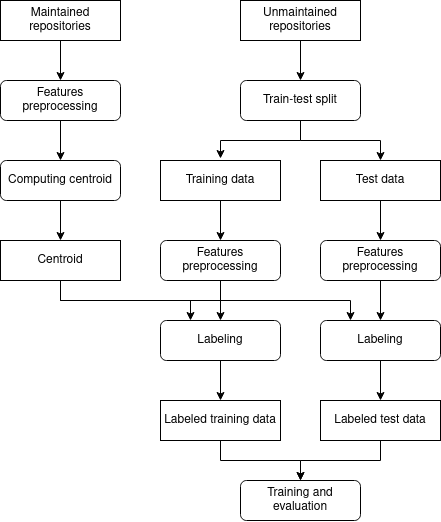
\includegraphics[scale=0.8]{chapters/chapter3/preprocessing.png}
    \caption{Scheme of preprocessing}
    \label{fig:preprocessing}
\end{figure}

\section{Samples labeling}
\label{sec:labeling}

Classification models are trained in a supervised manner, this means that the training data need to be labeled.
Labeling process is as follows:

\begin{enumerate}
    \item Gather a sufficient quantity of suitable repositories \ref{sec:filtering}.

    \item Cluster \emph{maintained} repositories and find their centroid using a KMeans algorithm\footnote{See \url{https://scikit-learn.org/stable/modules/generated/sklearn.cluster.KMeans.html}}.
    Centroid is central vector, which may not necessarily be a member of the data set.
    The centroid can be thought of as the multi-dimensional average of the cluster.

    \item Compute an \emph{l2}\footnote{See \url{https://scikit-learn.org/stable/modules/generated/sklearn.metrics.pairwise.euclidean_distances.html}} (Euclidean) distance of every \emph{unmaintained} repository from the \emph{maintained} repository cluster centroid.
    
    \item Create a subset of \emph{unmaintained} repositories with outliers removed.
    Outliers are determined using \emph{Interquartile range} approach\footnote{See \url{https://www.statology.org/find-outliers-with-iqr/}} computed on the Euclidean distances of repositories from the centroid.

    \item Based on this subset, 10 equally sized bins are created.

    \item Label all repositories based on the bin they belong to.
    Repositories with the distance greater than the limit of the last bin are put into that last bin, and repositories smaller than the limit of the smallest bin are put into the smallest one.
\end{enumerate}

Labeled train and test data are then used in the training and evaluation process \ref{sec:training_evaluation}.
% todo hodit histogram lablov

\section{Training and evaluation}
\label{sec:training_evaluation}

Four machine learning algorithms were tested for the best result, these are:

\begin{enumerate}
\label{sec:models}
    \item RandomForest\footnote{See \url{https://scikit-learn.org/stable/modules/generated/sklearn.ensemble.RandomForestClassifier.html}}
    \item SVC\footnote{See \url{https://scikit-learn.org/stable/modules/generated/sklearn.svm.SVC.html}}
    \item kNN\footnote{See \url{https://scikit-learn.org/stable/modules/generated/sklearn.neighbors.KNeighborsClassifier.html}}
    \item MLP\footnote{See \url{https://scikit-learn.org/stable/modules/generated/sklearn.neural_network.MLPClassifier.html}}
\end{enumerate}

Best set of hyper-parameters for models \ref{sec:models} were tuned using \emph{grid search}\footnote{See \url{https://scikit-learn.org/stable/modules/generated/sklearn.model_selection.GridSearchCV.html\#sklearn.model_selection.GridSearchCV}}.
Using \emph{grid search} technique, every possible combination of pre-defined hyper-parameters is tried and evaluated in order to find the set with the best performance.
Parameter grids used in the thesis can be seen in the tables \ref{tab:grid-rf}, \ref{tab:grid-knn}, \ref{tab:grid-svm} and \ref{tab:grid-mlp}.

Models are evaluated using 5-fold \emph{cross validation}\footnote{See \url{https://en.wikipedia.org/wiki/Cross-validation_(statistics)}}.
Two scores were used for evaluating quality of model's predictions.

\begin{enumerate}
    \item Accuracy - simple fraction of correct predictions and all predictions.

    \item Custom accuracy score with deviation:
    Very similar to accuracy score, but prediction label of one more or one less than the true label is still considered as a correct prediction.
    For example, true label is 7.
    If the model predicts 6, 7, or 8, all of these are considered a correct prediction.
    Number of correct predictions is then divided by the number of all predictions as usual.
    
    I added this score to compute accuracy with small deviation, if the user cares accepts a small error in predictions.
    
\end{enumerate}

% todo doplnint
\begin{table}
  \caption{Parameters grid for RandomForest}
  \label{tab:grid-rf}
  \begin{tabular}{|c|c|}
    \toprule
    Hyper-parameter & Values \\
    \midrule
    criterion & gini, entropy \\
    \bottomrule
  \end{tabular}
\end{table}

% todo doplnint
\begin{table}
  \caption{Parameters grid for SVM}
  \label{tab:grid-svm}
  \begin{tabular}{|c|c|}
    \toprule
    Hyper-parameter & Values \\
    \midrule
    criterion & gini, entropy \\
    \bottomrule
  \end{tabular}
\end{table}

% todo doplnint
\begin{table}
  \caption{Parameters grid for kNN}
  \label{tab:grid-knn}
  \begin{tabular}{|c|c|}
    \toprule
    Hyper-parameter & Values \\
    \midrule
    criterion & gini, entropy \\
    \bottomrule
  \end{tabular}
\end{table}

% todo doplnint
\begin{table}
  \caption{Parameters grid for MLP}
  \label{tab:grid-mlp}
  \begin{tabular}{|c|c|}
    \toprule
    Hyper-parameter & Values \\
    \midrule
    criterion & gini, entropy \\
    \bottomrule
  \end{tabular}
\end{table}
